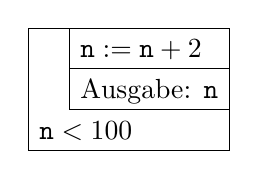
\begin{tikzpicture}
    \draw (0pt,0pt) rectangle (72.58547pt, -44.2243pt);
    \node at (4.0pt, -22.11215pt) {};
    \node at (20.79161pt, -37.19757pt) {$\texttt{n} < 100$};
    \draw (14.83542pt,0pt) rectangle (72.58547pt, -14.44444pt);
    \node at (40.751954999999995pt, -7.638885pt) {$\texttt{n} := \texttt{n} + 2$};
    \draw (14.83542pt,-14.44444pt) rectangle (72.58547pt, -29.38888pt);
    \node at (43.710445pt, -22.88888pt) {Ausgabe: $\texttt{n}$};
\end{tikzpicture}
